% ==============================================================
%  AutoNexa — FINAL REPORT
%  Autonomous Parking and Recall System
%
%  Single self-contained source. Compiles with pdfLaTeX (Overleaf).
%  Reuses the preamble/style of docs/AutoNexa_CDRR_Final.tex and brings
%  the technical content current to the delivered prototype:
%    - L298N H-bridge motor driver (not Hiwonder I2C)
%    - SMAC Hybrid-A* global + MPPI local controller (RPP fallback)
%    - ASCII nav2_pico_bridge as primary actuation path
%    - 12.8 V / 7 Ah lead-acid battery
%
%  EDITING NOTES
%   * Red [BRACKETED] text and <  > markers = fill in before submission.
%   * Search for "\TODO" and "\fillin" to find every blank.
%   * Performance-test tables (Ch. Results) and Budget tables expect the
%     team's measured numbers / actual prices.
% ==============================================================
\documentclass[12pt,a4paper]{report}

% -------------------- PACKAGES --------------------
\usepackage[utf8]{inputenc}
\usepackage[T1]{fontenc}
\usepackage{lmodern}
\usepackage[a4paper,top=2.5cm,bottom=2.5cm,left=2.5cm,right=2.5cm]{geometry}
\usepackage{setspace}
\usepackage{amsmath}
\usepackage{amssymb}
\usepackage{graphicx}
\usepackage{float}
\usepackage{array}
\usepackage{booktabs}
\usepackage{longtable}
\usepackage{tabularx}
\usepackage{multirow}
\usepackage{caption}
\usepackage{subcaption}
\usepackage{titlesec}
\usepackage{fancyhdr}
\usepackage{hyperref}
\usepackage{enumitem}
\usepackage{pdflscape}
\usepackage{appendix}
\usepackage{xcolor}
\usepackage{tikz}
\usepackage{listings}
\usetikzlibrary{arrows.meta,positioning,shapes.geometric,fit,calc}

% -------------------- HYPERREF --------------------
\hypersetup{
    colorlinks=true,
    linkcolor=blue,
    urlcolor=blue,
    citecolor=blue,
    pdftitle={AutoNexa Final Report},
    pdfauthor={AutoNexa Team},
    pdfsubject={Final Report},
    pdfkeywords={AutoNexa, Final Report, Autonomous Parking, ROS2, Nav2, SLAM}
}

% -------------------- LISTINGS (code/flow blocks) --------------------
\lstset{
    basicstyle=\ttfamily\small,
    breaklines=true,
    frame=single,
    backgroundcolor=\color{gray!8},
    rulecolor=\color{gray!40},
    xleftmargin=6pt,
    xrightmargin=6pt,
    aboveskip=6pt,
    belowskip=6pt
}

% -------------------- SPACING --------------------
\onehalfspacing

% -------------------- COLOURS --------------------
\definecolor{navyblue}{RGB}{26,46,74}
\definecolor{lightblue}{RGB}{220,232,245}

% -------------------- HEADER / FOOTER --------------------
\pagestyle{fancy}
\fancyhf{}
\fancyhead[L]{\textcolor{navyblue}{\textbf{AutoNexa}}}
\fancyhead[R]{\textcolor{navyblue}{Final Report}}
\fancyfoot[C]{\thepage}
\renewcommand{\headrulewidth}{0.4pt}

% -------------------- SECTION FORMATTING --------------------
\titleformat{\chapter}[display]
    {\bfseries\Large\color{navyblue}}
    {\chaptertitlename\ \thechapter}{10pt}{\Huge}

\titleformat{\section}
    {\bfseries\large\color{navyblue}}{\thesection}{1em}{}

\titleformat{\subsection}
    {\bfseries\normalsize}{\thesubsection}{1em}{}

\titleformat{\subsubsection}
    {\bfseries\normalsize\itshape}{\thesubsubsection}{1em}{}

% -------------------- CUSTOM COMMANDS --------------------
\newcommand{\pname}{AutoNexa}
\newcommand{\reportdate}{[Submission Date]}
\newcommand{\courseinfo}{EE493 / EE494}
\newcommand{\ver}{Final Report --- Version 1.0}
% Fill-in helpers: anything red must be completed before submission.
\newcommand{\TODO}[1]{\textcolor{red}{\textbf{[#1]}}}
\newcommand{\fillin}{\textcolor{red}{$\langle\ \rangle$}}

% ==============================================================
\begin{document}

% ==================== TITLE PAGE ====================
\begin{titlepage}
    \centering
    \vspace*{1.0cm}

    {\large \TODO{University Name} \par}
    \vspace{0.2cm}
    {\large \TODO{Faculty / Department of Electrical and Electronics Engineering} \par}

    \vspace{1.4cm}

    {\Huge \textbf{\textcolor{navyblue}{\pname}} \par}
    \vspace{0.4cm}
    {\LARGE Autonomous Parking and Recall System \par}
    \vspace{1.4cm}

    \noindent\rule{\textwidth}{1.5pt}
    \vspace{0.4cm}

    {\Huge \textbf{Final Report} \par}
    \vspace{0.4cm}
    \noindent\rule{\textwidth}{1.5pt}

    \vspace{1cm}
    {\Large \courseinfo \par}
    \vspace{0.3cm}
    {\large \ver \par}
    \vspace{0.3cm}
    {\large \reportdate \par}

    \vfill

    \begin{flushleft}
    \textbf{Design Studio Section:} \TODO{X} \\[0.3cm]
    \textbf{Supervisor:} \TODO{Title Name Surname} \\[0.3cm]
    \textbf{Team / Company:} AutoNexa \\[0.3cm]
    \textbf{Presented by:} \\[0.2cm]
    \quad An\i{}l Salih \c{C}olak \\
    \quad Do\u{g}ukan Zorlu \\
    \quad Emre Mende\c{s} \\
    \quad Ismayil Ibrahimli \\
    \quad Oghuz Novruzaliyev \\
    \quad Umut Kumral \\
    \end{flushleft}

    \vfill
\end{titlepage}

% ==================== FRONT MATTER ====================
\pagenumbering{roman}
\tableofcontents
\clearpage
\listoffigures
\clearpage
\listoftables
\clearpage

% ==================== COMPANY ORGANIZATION ====================
\chapter*{Company Organization}
\addcontentsline{toc}{chapter}{Company Organization}

\pname{} is organized as a flat engineering team of equal contributors with no
designated project lead; all members share collective responsibility for the
system and its integration. Within that shared model the only dedicated split is
the power and electrical subsystem, which was handled by two members, while the
remaining four members jointly developed the rest of the system (embedded
firmware, perception, navigation, the mobile application, and testing).

\begin{figure}[H]
\centering
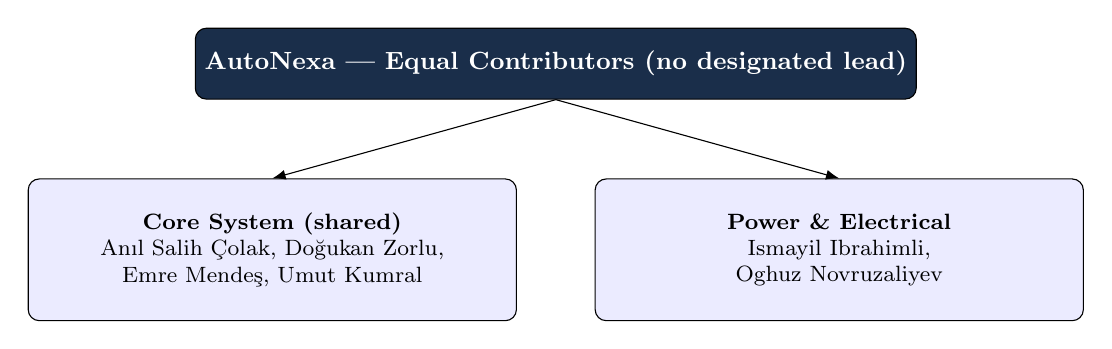
\begin{tikzpicture}[
    node distance=10mm and 12mm,
    team/.style={draw, rounded corners, fill=navyblue, text=white, font=\small\bfseries,
                 align=center, minimum width=8cm, minimum height=0.9cm},
    grp/.style={draw, rounded corners, fill=blue!8, font=\footnotesize,
                align=center, minimum width=6.2cm, minimum height=1.8cm},
    line/.style={-Latex}
]
\node[team] (team) {AutoNexa --- Equal Contributors (no designated lead)};
\node[grp, below=of team, xshift=-3.6cm] (core)
     {\textbf{Core System (shared)}\\\normalfont An\i{}l Salih \c{C}olak,
      Do\u{g}ukan Zorlu,\\\normalfont Emre Mende\c{s}, Umut Kumral};
\node[grp, below=of team, xshift=3.6cm] (pwr)
     {\textbf{Power \& Electrical}\\\normalfont Ismayil Ibrahimli,\\\normalfont
      Oghuz Novruzaliyev};
\draw[line] (team.south) -- (core.north);
\draw[line] (team.south) -- (pwr.north);
\end{tikzpicture}
\caption{\pname{} team / company organization chart (flat, shared responsibility).}
\label{fig:org}
\end{figure}

\noindent\textit{Note: all members contributed with equal responsibility; the
table records only the work-area split (power vs.\ shared core system).}

\begin{table}[H]
\centering
\caption{Team members and work-area split.}
\label{tab:roles}
\begin{tabularx}{\textwidth}{|p{4.2cm}|p{3.4cm}|X|}
\hline
\textbf{Member} & \textbf{Work Area} & \textbf{Notes} \\
\hline
Ismayil Ibrahimli & Power \& Electrical & Battery, power distribution, regulators, wiring \\
\hline
Oghuz Novruzaliyev & Power \& Electrical & Battery, power distribution, regulators, wiring \\
\hline
An\i{}l Salih \c{C}olak & Core system (shared) & Embedded, perception, navigation, app, and integration shared equally across the four \\
\hline
Do\u{g}ukan Zorlu & Core system (shared) & Embedded, perception, navigation, app, and integration shared equally across the four \\
\hline
Emre Mende\c{s} & Core system (shared) & Embedded, perception, navigation, app, and integration shared equally across the four \\
\hline
Umut Kumral & Core system (shared) & Embedded, perception, navigation, app, and integration shared equally across the four \\
\hline
\end{tabularx}
\end{table}

% ==================== EXECUTIVE SUMMARY ====================
\chapter*{Executive Summary}
\addcontentsline{toc}{chapter}{Executive Summary}

\pname{} is a small-scale autonomous parking and recall robot for structured
indoor environments. It builds a map of its surroundings live, localizes itself,
plans collision-aware paths to a parking or recall target, and executes safe
low-speed Ackermann maneuvers through a multi-layer safety pipeline. The system
is built around a Raspberry Pi~5 running ROS~2 Jazzy for high-level autonomy, a
Raspberry Pi Pico for deterministic low-level actuation, and a SLAMTEC~C1 2D
LiDAR as the primary sensing device. An accompanying Flutter mobile application
serves as a full operator console, because the deployed robot typically runs
headless (no monitor or RViz on site).

This Final Report documents the completed design effort. Since the Critical
Design Review, the platform progressed from a subsystem-validated prototype to an
integrated vehicle. Several design decisions matured during integration: the
motor driver was changed from a smart I2C unit to a robust L298N H-bridge after a
hardware failure; the navigation stack was upgraded from a differential-drive
planner/controller pair to a kinematically correct \mbox{SMAC Hybrid-A*} global
planner with a sampling-based Model Predictive Path Integral (MPPI) local
controller (with Regulated Pure Pursuit retained as a no-rebuild fallback); the
actuation transport was consolidated onto a hardened ASCII serial bridge; and the
mobile app grew into a complete operator console with manual safety bypass,
direction calibration, live tuning, and waypoint management.

The system delivers: live SLAM mapping and navigation with no pre-saved map
required; a seven-layer safety stack culminating in a latching hardware E-STOP;
an open-loop Ackermann chassis with quadrature-encoder feedback; and a wireless
operator console. Headline measured performance ---
parking accuracy, endurance, and control-loop timing --- is summarized in
Chapter~\ref{ch:results} (\TODO{insert one-line headline result once data is in,
e.g. ``final parking error within $\pm$X\,cm over N trials''}).

The remaining open items --- IMU-assisted odometry fusion, formal long-duration
soak testing, and camera-guided final-approach docking --- are additive
extensions that the modular architecture supports without redesign. The full
deliverable set, user manual, budget, and design discussions follow.

% ==================== CHAPTER 1: INTRODUCTION ====================
\chapter{Introduction}

\section{Problem Statement and Motivation}

Parking in constrained indoor spaces is slow, repetitive, and error-prone for
human drivers, and it consumes a disproportionate share of low-speed maneuvering
time and floor area. \pname{} addresses a scaled-down version of this problem: a
vehicle that can autonomously survey a small structured environment, drive itself
to a designated parking slot, and later return (``recall'') to a user-defined
location on command --- all while guaranteeing safe behavior at every layer of
the control stack.

\section{Objectives}

\begin{itemize}[leftmargin=1.4cm]
    \item Autonomous low-speed navigation in a constrained indoor parking area
          without a pre-saved map.
    \item Precise final parking pose with a small position tolerance.
    \item Summon / recall to a stored location.
    \item A safety architecture in which no planner output can reach the motors
          without passing through independent software and hardware safety stages.
    \item A wireless operator interface usable without a monitor or desktop tools.
\end{itemize}

\section{Scope}

The delivered system covers perception (LiDAR-based mapping and localization),
navigation (global planning and local control with obstacle avoidance), embedded
actuation (Ackermann steering and rear-wheel drive), a layered safety system, and
a mobile operator console. Camera-guided ArUco docking and IMU-fused odometry are
designed-in and partially staged but are documented as planned extensions rather
than fully validated capabilities.

\section{Organization of the Report}

Chapter~\ref{ch:design} gives the top-down system design. Chapters~\ref{ch:embedded}--\ref{ch:appcomms}
detail the embedded, perception, navigation, and software/application subsystems.
Chapter~\ref{ch:standards} lists the engineering standards applied and the design
changes since the CDR. Chapter~\ref{ch:results} presents performance-test results.
Chapter~\ref{ch:deliverables} lists the deliverables, Chapter~\ref{ch:budget} the
budget, and Chapter~\ref{ch:discussion} the required discussions on safety,
societal impact, and environmental effects. The user manual and supporting data
are in the appendices.

% ==================== CHAPTER 2: SYSTEM DESIGN ====================
\chapter{System Design Description}
\label{ch:design}

\section{Overall System Description}

The architecture is a strictly layered perception-to-actuation chain with no
direct coupling between high-level planning and hardware. LiDAR data drives both
mapping and odometry. Nav2 produces motion requests that are never sent directly
to the motors; they must pass through a velocity smoother, a collision monitor,
and a bridge layer before reaching the Pico. The Pico itself applies a final
hardware-level watchdog and a latching E-STOP independently of the Raspberry~Pi~5
software.

\section{System-Level Block Diagram}

\begin{figure}[H]
\centering
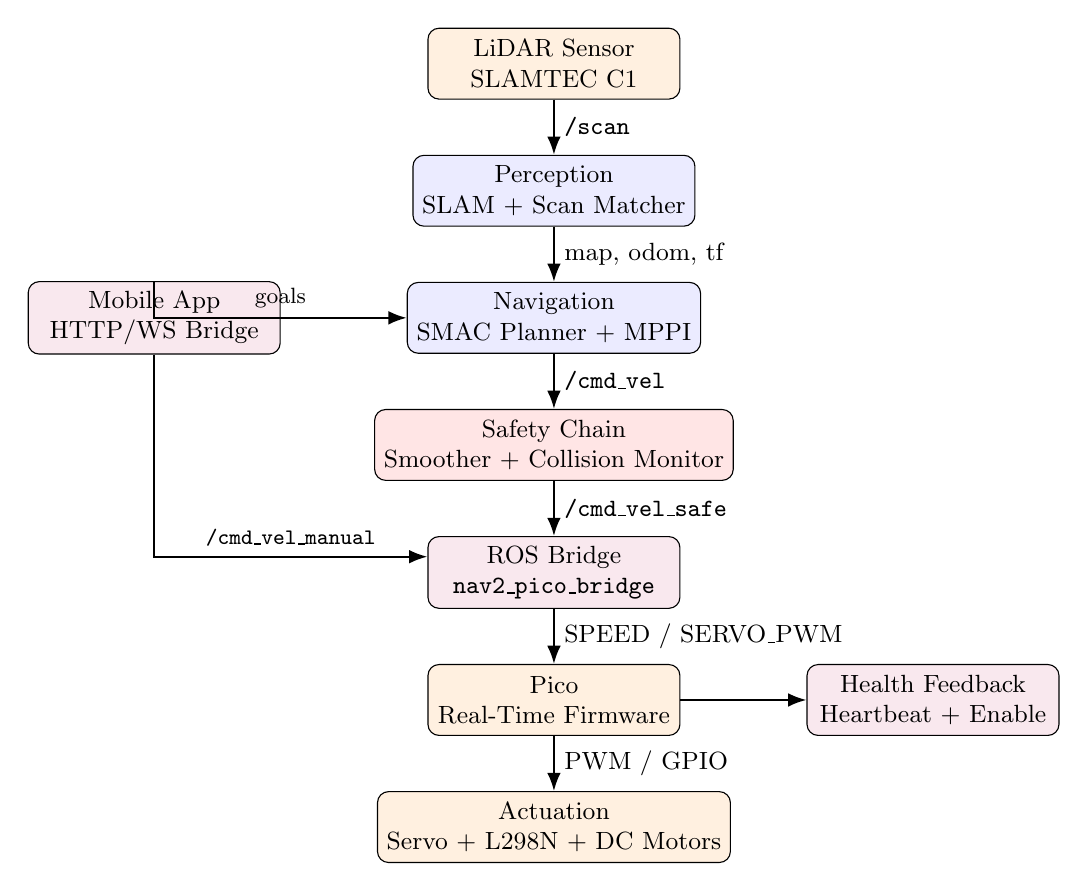
\begin{tikzpicture}[
    node distance=7mm and 16mm,
    block/.style={draw, rounded corners, minimum width=3.2cm, minimum height=0.9cm,
                  align=center, fill=blue!8, font=\small},
    safety/.style={draw, rounded corners, minimum width=3.2cm, minimum height=0.9cm,
                   align=center, fill=red!10, font=\small},
    hw/.style={draw, rounded corners, minimum width=3.2cm, minimum height=0.9cm,
               align=center, fill=orange!12, font=\small},
    io/.style={draw, rounded corners, minimum width=3.2cm, minimum height=0.9cm,
               align=center, fill=purple!9, font=\small},
    line/.style={-Latex, thick}
]
\node[hw]      (lidar)      {LiDAR Sensor\\SLAMTEC C1};
\node[block,   below=of lidar]   (percep)  {Perception\\SLAM + Scan Matcher};
\node[block,   below=of percep]  (nav2)    {Navigation\\SMAC Planner + MPPI};
\node[safety,  below=of nav2]    (safety)  {Safety Chain\\Smoother + Collision Monitor};
\node[io,      below=of safety]  (bridge)  {ROS Bridge\\\texttt{nav2\_pico\_bridge}};
\node[hw,      below=of bridge]  (pico)    {Pico\\Real-Time Firmware};
\node[hw,      below=of pico]    (act)     {Actuation\\Servo + L298N + DC Motors};
\node[io,      right=of pico]    (health)  {Health Feedback\\Heartbeat + Enable};
\node[io,      left=of nav2]     (app)     {Mobile App\\HTTP/WS Bridge};

\draw[line] (lidar)  -- node[right,font=\small]{\texttt{/scan}}        (percep);
\draw[line] (percep) -- node[right,font=\small]{map, odom, tf}          (nav2);
\draw[line] (nav2)   -- node[right,font=\small]{\texttt{/cmd\_vel}}    (safety);
\draw[line] (safety) -- node[right,font=\small]{\texttt{/cmd\_vel\_safe}} (bridge);
\draw[line] (bridge) -- node[right,font=\small]{SPEED / SERVO\_PWM} (pico);
\draw[line] (pico)   -- node[right,font=\small]{PWM / GPIO}             (act);
\draw[line] (pico.east)   -- (health.west);
\draw[line] (app.south) |- ([yshift=2mm]bridge.west) node[pos=0.75,above,font=\footnotesize]{\texttt{/cmd\_vel\_manual}};
\draw[line] (app.north) |- (nav2.west) node[pos=0.75,above,font=\footnotesize]{goals};
\end{tikzpicture}
\caption{System-level block diagram of the \pname{} platform (delivered configuration).}
\label{fig:system_block}
\end{figure}

\section{Main Data and Control Signals}

\begin{table}[H]
\centering
\caption{Key ROS~2 topics and their roles in the system.}
\label{tab:signals}
\begin{tabularx}{\textwidth}{|p{3.4cm}|p{2.2cm}|p{2.8cm}|X|}
\hline
\textbf{Topic} & \textbf{Type} & \textbf{Source $\rightarrow$ Sink} & \textbf{Purpose} \\
\hline
\texttt{/scan} & \texttt{LaserScan} & LiDAR $\rightarrow$ SLAM, Nav2 & Raw and filtered environment sensing \\
\hline
\texttt{/map} & \texttt{OccupancyGrid} & SLAM Toolbox $\rightarrow$ Nav2 & Live occupancy map (2\,cm/pixel) \\
\hline
\texttt{/odom} & \texttt{Odometry} & Scan matcher $\rightarrow$ Nav2 & Incremental pose estimate (ICP) \\
\hline
\texttt{/cmd\_vel} & \texttt{Twist} & Nav2 $\rightarrow$ smoother & Raw motion command \\
\hline
\texttt{/cmd\_vel\_smoothed} & \texttt{Twist} & Smoother $\rightarrow$ monitor & Acceleration-shaped command \\
\hline
\texttt{/cmd\_vel\_safe} & \texttt{Twist} & Collision monitor $\rightarrow$ bridge & Safety-filtered autonomous command \\
\hline
\texttt{/cmd\_vel\_manual} & \texttt{Twist} & App $\rightarrow$ bridge & Manual safety-bypass joystick command \\
\hline
\texttt{/pico/joint\_feedback} & \texttt{JointState} & Pico $\rightarrow$ RPi5 & Wheel velocities + steering angle \\
\hline
\texttt{/pico/odom} & \texttt{Odometry} & Pico $\rightarrow$ RPi5 & Encoder odometry (not yet fused into TF) \\
\hline
\texttt{/tf}, \texttt{/tf\_static} & TF transforms & Multiple nodes & Frame consistency \\
\hline
\end{tabularx}
\end{table}

\section{System and Subsystem Requirements}

\subsection{System-Level Requirements}

\begin{table}[H]
\centering
\caption{System-level requirements.}
\label{tab:sys_req}
\begin{tabularx}{\textwidth}{|p{1.7cm}|X|p{3.2cm}|}
\hline
\textbf{ID} & \textbf{Requirement} & \textbf{Target} \\
\hline
SYS-01 & Autonomous navigation in a constrained indoor parking environment & Functional completion \\
\hline
SYS-02 & Safe low-speed operation & $\leq$ 0.5 m/s; $\sim$0.1 m/s final approach \\
\hline
SYS-03 & Precise autonomous parking & Final position error within tolerance \\
\hline
SYS-04 & Summon / recall operation & Return to user-defined location on command \\
\hline
SYS-05 & Collision-aware command output & No unsafe direct path planner $\rightarrow$ actuators \\
\hline
SYS-06 & Safe stop on command loss & Timeout $\leq$ 200 ms \\
\hline
SYS-07 & Deterministic command update & 30 Hz nominal bridge publish rate \\
\hline
SYS-08 & Obstacle detection & Static and dynamic obstacles in costmap \\
\hline
SYS-09 & Wireless user interaction & Mobile app control at usable range \\
\hline
SYS-10 & Power endurance & All subsystems operational for $\geq$ 15 min \\
\hline
\end{tabularx}
\end{table}

\subsection{Subsystem Requirements}

\begin{table}[H]
\centering
\caption{Localization, navigation, and control subsystem requirements.}
\label{tab:sub_req}
\begin{tabularx}{\textwidth}{|p{3cm}|X|}
\hline
\textbf{Subsystem} & \textbf{Key Requirements} \\
\hline
Localization & Resolve geometric features at $\geq$ 2 cm; pose update $\geq$ 10 Hz; detect obstacles as close as 0.05 m; consistent map after repeated passes. \\
\hline
Navigation & Generate a collision-free path to a valid goal; respect Ackermann (minimum turning radius) constraints; operate in narrow indoor lanes without blocking localization. \\
\hline
Control & Convert body velocity to steering angle and wheel speeds (Ackermann); execute commands at $\geq$ 30 Hz; stop motors within 200 ms of command loss; latch E-STOP independently of the software stack; saturate velocity and acceleration before actuation. \\
\hline
\end{tabularx}
\end{table}

\section{System Operation Overview}

\begin{enumerate}[label=\textbf{Step \arabic*:}, leftmargin=2.5cm]
    \item \textbf{Sensing.} The LiDAR scans the environment at $\sim$10 Hz over
          360\textdegree{}; data is filtered and published as \texttt{/scan}.
    \item \textbf{Localization and Mapping.} SLAM Toolbox builds a live occupancy
          map and the laser scan matcher estimates pose by ICP.
    \item \textbf{Decision-Making.} Nav2 plans a global path (SMAC Hybrid-A*) and
          computes local velocity commands (MPPI) toward the goal.
    \item \textbf{Command Conditioning.} The velocity smoother shapes acceleration
          and the collision monitor checks a forward trajectory; output is
          \texttt{/cmd\_vel\_safe}.
    \item \textbf{Bridge and Final Safety.} \texttt{nav2\_pico\_bridge} clamps
          velocity, limits acceleration and steering slew rate, applies a 200 ms
          timeout, and writes ASCII actuator commands over USB serial.
    \item \textbf{Actuation.} The Pico applies Ackermann inverse kinematics and
          drives the servo and rear motors; the hardware watchdog and E-STOP are
          enforced independently at this stage.
\end{enumerate}

\noindent In summary: \textbf{sensing $\rightarrow$ localization $\rightarrow$
planning $\rightarrow$ command conditioning $\rightarrow$ actuation}.

% ==================== CHAPTER 3: EMBEDDED SUBSYSTEM ====================
\chapter{Embedded Subsystem}
\label{ch:embedded}

\section{Overview}

The embedded subsystem runs on a Raspberry Pi Pico (RP2040, dual ARM
Cortex-M0+) and sits at the bottom of the software stack. It translates velocity
commands into physical actuator outputs and enforces hardware-level safety
independently of the Raspberry Pi 5. The firmware is written in C with the Pico
SDK and no RTOS; a single 50 Hz hardware-timer loop is the only scheduling
primitive. One source tree builds two targets (Table~\ref{tab:pico_builds}).

\begin{table}[H]
\centering
\caption{Pico firmware build targets.}
\label{tab:pico_builds}
\begin{tabularx}{\textwidth}{|p{4.8cm}|X|}
\hline
\textbf{Target} & \textbf{Purpose} \\
\hline
\texttt{autonexa\_pico.uf2} & ASCII serial CLI --- the \textbf{delivered actuation path}, driven by \texttt{nav2\_pico\_bridge.py} and bench-tested with \texttt{test/pico\_gui.py}. \\
\hline
\texttt{autonexa\_pico\_uros.uf2} & micro-ROS client (XRCE-DDS over USB CDC) --- alternative transport that exposes the Pico as native ROS~2 topics. \\
\hline
\end{tabularx}
\end{table}

\section{Hardware Interfaces and Pinout}

The motor driver is an \textbf{L298N} dual H-bridge, adopted after the previous
Hiwonder I2C smart driver failed. The L298N is a ``dumb'' driver: two direction
pins plus one PWM enable per motor. Quadrature Hall encoders on both rear motors
are read directly by the Pico through a PIO quadrature decoder, providing wheel
feedback for odometry even though motor control itself is open-loop.

\begin{table}[H]
\centering
\caption{Pico hardware interface and GPIO assignment (delivered build).}
\label{tab:pico_hw}
\begin{tabularx}{\textwidth}{|p{3.2cm}|p{3.6cm}|X|}
\hline
\textbf{Function} & \textbf{GPIO} & \textbf{Target / Notes} \\
\hline
Right motor direction & GP2 (IN1), GP3 (IN2) & L298N, OUT1--OUT2 \\
\hline
Right motor PWM enable & GP4 (ENA) & 10 kHz PWM \\
\hline
Left motor direction & GP6 (IN3), GP7 (IN4) & L298N, OUT3--OUT4 \\
\hline
Left motor PWM enable & GP8 (ENB) & 10 kHz PWM \\
\hline
Steering servo & GP15 & LD-1501MG, 50 Hz, 500--2500 $\mu$s \\
\hline
Left encoder A/B & GP10 / GP11 & PIO quadrature decoder \\
\hline
Right encoder A/B & GP12 / GP13 & PIO quadrature decoder \\
\hline
Heartbeat LED & GP25 & 1 Hz normal, 5 Hz = E-STOP latched \\
\hline
Host communications & USB CDC & Raspberry Pi 5 at 115{,}200 baud \\
\hline
\end{tabularx}
\end{table}

\section{Vehicle Parameters}

All physical constants are defined in \texttt{pico\_firmware/include/config.h}.

\begin{table}[H]
\centering
\caption{Vehicle physical and control parameters.}
\label{tab:vehicle_params}
\begin{tabularx}{\textwidth}{|p{5.0cm}|p{3.2cm}|X|}
\hline
\textbf{Parameter} & \textbf{Value} & \textbf{Notes} \\
\hline
Wheelbase $L$ & 0.25 m & Front-to-rear axle distance \\
\hline
Track width & 0.20 m & Left-to-right wheel centreline \\
\hline
Wheel radius $r$ & 0.033 m & 66 mm diameter \\
\hline
Max steering angle $\delta_{\max}$ & $\pm$30\textdegree{} ($\pm$0.5236 rad) & Servo-linkage limit \\
\hline
Motor gear ratio & 1:30 & JGB37-520R30, 12 V DC \\
\hline
Encoder edges per wheel rev & 1320 & $11 \times 4 \times 30$ \\
\hline
Control loop rate & 50 Hz (20 ms) & Hardware timer \\
\hline
Command timeout & 200 ms & Watchdog threshold \\
\hline
Motor PWM frequency & 10 kHz & Above audible range \\
\hline
Start-up duty floor & 60\% kick $\rightarrow$ 30\% sustain & Static-friction kick-start \\
\hline
\end{tabularx}
\end{table}

\section{Ackermann Kinematics and Related Calculations}

ROS~2 sends body-frame velocity commands $(v_x,\ \omega_z)$. The firmware
implements both directions of the Ackermann (bicycle) model.

\subsection{Inverse Kinematics (command $\rightarrow$ actuators)}

For a non-zero forward velocity, the required steering angle and turning radius
are
\begin{equation}
\delta = \arctan\!\left(\frac{L\,\omega_z}{v_x}\right),
\qquad
R = \frac{L}{\tan \delta},
\end{equation}
and the left/right rear-wheel speeds for a turn of radius $R$ are
\begin{equation}
v_{L} = v_x\left(1 - \frac{T}{2R}\right),
\qquad
v_{R} = v_x\left(1 + \frac{T}{2R}\right),
\end{equation}
where $T = 0.20$ m is the track width. Straight-line motion is the degenerate
case $\delta = 0,\ v_L = v_R = v_x$.

\subsection{Forward Kinematics (encoders $\rightarrow$ odometry)}

Each 20 ms cycle, encoder edge deltas are converted to wheel velocities and
integrated into an $(x, y, \psi)$ pose using
\begin{equation}
\bar{v} = \frac{v_L + v_R}{2},
\qquad
\dot{\psi} = \frac{\bar{v}\,\tan\delta}{L},
\qquad
\begin{cases}
\dot{x} = \bar{v}\cos\psi \\
\dot{y} = \bar{v}\sin\psi
\end{cases}
\end{equation}
published on \texttt{/pico/odom} at 20 Hz.

\subsection{Worked Design Values}

\begin{itemize}[leftmargin=1.4cm]
    \item \textbf{Minimum turning radius.}
          $R_{\min} = L / \tan\delta_{\max} = 0.25 / \tan 30\textdegree
          = 0.433$ m (geometric). The navigation stack uses a conservative
          $0.50$ m to leave margin for linkage slop.
    \item \textbf{Encoder linear resolution.} Wheel circumference
          $= 2\pi r = 0.207$ m; with 1320 edges/rev the distance per edge is
          $0.207 / 1320 \approx 0.157$ mm --- well below the 2 cm map cell.
    \item \textbf{Servo angle-to-pulse mapping.} Linear about centre:
          $t_{\mu s} = t_{\text{center}} + (\delta / \delta_{\max})\,\Delta t$,
          with the firmware range 500--2500 $\mu$s and the delivered ASCII bridge
          calibrated to centre 1650 $\mu$s, bounds 1100--1900 $\mu$s for this
          chassis.
\end{itemize}

\section{Control Loop}

\begin{lstlisting}
[50 Hz timer tick]
  |
  v
1. Read encoders       -- PIO quadrature decode (left + right)
  |
  v
2. Forward kinematics  -- edge deltas -> wheel velocities -> integrate odom
  |
  v
3. Safety check        -- timeout counter, E-STOP latch, heartbeat LED
  |
  v
4. Apply actuators     -- gated by safety_is_ok()
   - Steering angle -> servo PWM (GP15, 50 Hz)
   - Wheel speeds   -> L298N direction pins + PWM enable (10 kHz)
  |
  v
5a. ASCII CLI mode:              | 5b. micro-ROS mode:
    parse SPEED / SERVO_PWM      |     spin subscribers
    emit TEL telemetry @ 10 Hz   |     publish /pico/odom @ 20 Hz
\end{lstlisting}

\section{Safety System}

All actuator writes are gated through \texttt{safety\_is\_ok()}. Two independent
conditions block actuation, summarized in Table~\ref{tab:pico_safety}.

\begin{table}[H]
\centering
\caption{Embedded safety states and behaviors.}
\label{tab:pico_safety}
\begin{tabularx}{\textwidth}{|p{2.2cm}|p{2.5cm}|p{1.8cm}|p{2.4cm}|X|}
\hline
\textbf{State} & \textbf{Cause} & \textbf{Motors} & \textbf{LED} & \textbf{Recovery} \\
\hline
Normal & --- & Running & 1 Hz blink & --- \\
\hline
Timed out & No command for 200 ms & Stopped + centred & 1 Hz blink & Next valid command \\
\hline
E-STOP & Explicit trigger & Stopped + centred & 5 Hz blink & Explicit clear only \\
\hline
\end{tabularx}
\end{table}

The E-STOP is a latching flag; it does not self-recover, because a stop triggered
during motion should require deliberate human action to clear.

\section{Known Limitations}

\begin{table}[H]
\centering
\caption{Embedded subsystem open items.}
\label{tab:pico_limits}
\begin{tabularx}{\textwidth}{|p{4.2cm}|p{1.4cm}|X|}
\hline
\textbf{Item} & \textbf{Severity} & \textbf{Resolution Path} \\
\hline
Open-loop motor control (no PID on wheel speed) & Medium & Encoders are wired; closed-loop speed control is a firmware extension \\
\hline
Pico odometry not fused into TF & Medium & Integrate as EKF input when IMU is connected \\
\hline
No motor stall / overcurrent detection & Low & Hardware addition; out of current scope \\
\hline
\end{tabularx}
\end{table}

% ==================== CHAPTER 4: PERCEPTION SUBSYSTEM ====================
\chapter{Perception Subsystem}
\label{ch:perception}

\section{Overview}

The perception subsystem builds a real-time geometric model of the environment
and produces the pose estimate that everything downstream depends on. The design
is \textbf{LiDAR-first}: the 2D rotating LiDAR is the sole source of both mapping
(SLAM Toolbox) and incremental dead-reckoning (laser scan matching). A camera
(IMX219) is mounted and defined in the URDF for future ArUco-guided docking; it
does not participate in the SLAM or TF chain.

\section{SLAMTEC C1 LiDAR}

\begin{table}[H]
\centering
\caption{SLAMTEC C1 LiDAR specifications and ROS~2 integration.}
\label{tab:lidar_specs}
\begin{tabularx}{\textwidth}{|p{4.2cm}|X|}
\hline
\textbf{Property} & \textbf{Value} \\
\hline
Measurement principle & Rotating 2D laser ranging \\
\hline
Field of view & 360\textdegree{} \\
\hline
Operational range (configured) & 0.05 m -- 4.0 m \\
\hline
Scan frequency & $\sim$10 Hz \\
\hline
ROS~2 driver & \texttt{sllidar\_ros2} \\
\hline
Published topic / frame & \texttt{/scan} (\texttt{LaserScan}) / \texttt{laser\_link} \\
\hline
Serial interface & USB CDC at 460{,}800 baud \\
\hline
Physical mounting & +150 mm fwd, +120 mm above \texttt{base\_link} \\
\hline
\end{tabularx}
\end{table}

\noindent\textbf{Known failure mode.} If \texttt{sllidar\_node} is killed without
a clean shutdown, the OS may not release \texttt{/dev/ttyUSB0} and the next launch
returns \texttt{SL\_RESULT\_OPERATION\_TIMEOUT}. The fix is to kill stale
processes and use the deterministic \texttt{/dev/serial/by-id/} path.

\section{Scan Filter Chain}

Raw \texttt{/scan} passes through a four-stage \texttt{laser\_filters} chain
before SLAM or costmaps consume it.

\begin{table}[H]
\centering
\caption{Laser scan filter chain stages.}
\label{tab:filters}
\begin{tabularx}{\textwidth}{|p{0.5cm}|p{3.6cm}|p{3.2cm}|X|}
\hline
\textbf{\#} & \textbf{Filter} & \textbf{Key Parameters} & \textbf{Purpose} \\
\hline
1 & Range filter & 0.05--4.0 m & Remove out-of-range returns \\
\hline
2 & Shadow filter & 10\textdegree--170\textdegree{} & Remove grazing-angle ghost points \\
\hline
3 & Median filter & window 5 & Suppress flicker on reflective surfaces \\
\hline
4 & Outlier filter & 0.5 m / win 5 & Remove isolated multi-path spikes \\
\hline
\end{tabularx}
\end{table}

\section{Odometry --- Laser Scan Matcher}

All incremental dead-reckoning is performed by ICP scan-to-scan matching
(\texttt{ros2\_laser\_scan\_matcher}), which publishes \texttt{/odom} and the
\texttt{odom$\rightarrow$base\_link} transform. Keyframes are created after
0.10 m of translation or 10\textdegree{} of rotation. Drift accumulates slowly;
for the few-metre parking maneuvers it is negligible, and IMU fusion is the
planned long-run mitigation.

\section{SLAM Toolbox --- Live Mapping}

SLAM Toolbox runs in asynchronous mapping mode; there is no pre-loaded map. Key
parameters: 0.02 m/pixel resolution (a $0.5\times1.0$ m slot $= 25\times50$
cells), map update after 0.05 m or 0.05 rad of motion, loop-closure search radius
3.0 m, and \texttt{provide odometry frame: false} so the scan matcher owns
\texttt{odom$\rightarrow$base\_link}. A localization mode against a pre-saved map
(AMCL) is also available as an alternative launch.

\section{TF Tree}

\begin{lstlisting}
map
 |  <-- SLAM Toolbox (map-level correction; AMCL in localization mode)
 v
odom
 |  <-- laser_scan_matcher (incremental dead-reckoning, ~10 Hz)
 v
base_link
 |  <-- robot_state_publisher (fixed sensor placement)
 v
laser_link
\end{lstlisting}

The \texttt{odom$\rightarrow$base\_link} transform never jumps, guaranteeing
smooth velocity commands; SLAM Toolbox adjusts \texttt{map$\rightarrow$odom} to
keep the global pose consistent.

\section{Known Limitations}

\begin{table}[H]
\centering
\caption{Perception subsystem open items.}
\label{tab:perc_limits}
\begin{tabularx}{\textwidth}{|p{3.8cm}|p{1.4cm}|X|}
\hline
\textbf{Item} & \textbf{Severity} & \textbf{Resolution Path} \\
\hline
Scan-only odometry drift on long runs & Medium & IMU + EKF fusion (staged) \\
\hline
LiDAR serial-port lock on hard kill & Medium & by-id path + preflight kill check \\
\hline
ICP weak in featureless corridors & Low & Limit angular velocity; IMU bridges gaps \\
\hline
Camera not yet integrated into ROS & Low & URDF + app ready; ROS image node pending \\
\hline
\end{tabularx}
\end{table}

% ==================== CHAPTER 5: NAVIGATION SUBSYSTEM ====================
\chapter{Navigation Subsystem}
\label{ch:navigation}

\section{Overview}

The navigation subsystem takes a goal pose --- from RViz or the mobile app ---
and produces velocity commands that move the robot to that goal while avoiding
obstacles, using the ROS~2 Nav2 stack on top of the live SLAM map. Navigation
requests can be sent as soon as the TF tree is healthy.

\section{Global Planner --- SMAC Hybrid-A*}

The global planner is \texttt{SmacPlannerHybrid}, a kinematically aware Hybrid-A*
that plans in $(x, y, \theta)$ and respects a minimum turning radius. It uses the
\texttt{REEDS\_SHEPP} motion model with \texttt{allow\_reversing: true}, so it can
generate forward/reverse (K-turn / back-in) maneuvers appropriate for parking.
\texttt{allow\_unknown} is \texttt{false}: the robot will not plan into unmapped
space, so the operator surveys the area first.

\section{Local Controller --- MPPI (default) / RPP (fallback)}

The local controller is \textbf{switchable at launch} via the \texttt{controller}
argument, with no rebuild required.

\subsection{MPPIController (default)}

MPPI (Model Predictive Path Integral) samples a batch of candidate trajectories
each control tick, rolls them through the Ackermann motion model, and scores them
against the costmap with a set of weighted critics. Unlike a pure-pursuit
controller it keeps clearance from walls \emph{while continuing to drive}, which
is why the autonomous chain can rely on it (plus the bridge clamps and hardware
watchdog) for obstacle safety.

\begin{table}[H]
\centering
\caption{MPPI controller key parameters (\texttt{config/controller\_mppi.yaml}).}
\label{tab:mppi}
\begin{tabularx}{\textwidth}{|p{5.2cm}|p{2.6cm}|X|}
\hline
\textbf{Parameter} & \textbf{Value} & \textbf{Notes} \\
\hline
Controller frequency & 10 Hz & \texttt{model\_dt} $= 1/f = 0.1$ s \\
\hline
Time steps / horizon & 40 / 4.0 s & $\text{horizon} = \text{steps}\times\text{model\_dt}$ \\
\hline
Batch size & 1000 & Primary Pi-5 CPU knob \\
\hline
Motion model & Ackermann & \texttt{min\_turning\_r} 0.50 m \\
\hline
$v_x$ max / min & 0.10 / $-$0.10 m/s & Reverse allowed; live-tunable via app slider \\
\hline
$\omega_z$ max & 0.50 rad/s & In lockstep with velocity smoother \\
\hline
Critics & 8 & Constraint, Cost, Goal, GoalAngle, PreferForward, PathAlign, PathFollow, PathAngle \\
\hline
\end{tabularx}
\end{table}

MPPI is the heaviest Nav2 node. A benchmark gate on the Pi~5 (controller CPU and
achieved \texttt{/cmd\_vel} rate) precedes trusting its tuning; a documented
back-off ladder (\texttt{batch\_size} $\rightarrow$ \texttt{time\_steps}
$\rightarrow$ \texttt{controller\_frequency}) keeps the rate $\geq 8$ Hz, and
\texttt{controller:=rpp} is the escape hatch.

\subsection{Regulated Pure Pursuit (fallback)}

RPP is a lighter geometric controller retained for the case where MPPI cannot
hold rate on the Pi. Representative tuning: \texttt{desired\_linear\_vel}
0.15 m/s, \texttt{max\_vel\_theta} 0.50 rad/s, lookahead 0.40 m (0.30--0.60 m),
goal tolerance 0.15 m / 0.10 rad.

\section{Costmaps}

Both costmaps use 0.02 m/cell resolution to match the SLAM map and avoid
resampling artifacts. The local costmap is a $2\times2$ m rolling window
(obstacle + inflation layers, $\sim$0.20 m inflation); the global costmap covers
the full map (static + obstacle + inflation, $\sim$0.15 m inflation).

\section{Velocity Pipeline and Safety Chain}

\begin{lstlisting}
Controller (MPPI/RPP)   /cmd_vel (~10 Hz)
        |
        v
Velocity Smoother       /cmd_vel_smoothed (20 Hz)  -- accel shaping
        |
        v
Collision Monitor       /cmd_vel_safe              -- forward trajectory check
        |
        v
nav2_pico_bridge        SPEED / SERVO_PWM (30 Hz)  -- clamp + accel cap
  (also subscribes /cmd_vel_manual for manual bypass)   + steer slew + 200 ms timeout
        |
        v
USB CDC serial (115200 baud)
        |
        v
Pico firmware (50 Hz)  ->  Servo + L298N + Motors
\end{lstlisting}

\section{End-to-End Latency}

\begin{table}[H]
\centering
\caption{Navigation pipeline update rates and latency contributions.}
\label{tab:latency}
\begin{tabularx}{\textwidth}{|p{5.2cm}|p{2.4cm}|X|}
\hline
\textbf{Stage} & \textbf{Rate} & \textbf{Typical Latency} \\
\hline
LiDAR scan & $\sim$10 Hz & $<$100 ms \\
\hline
Scan filter + matcher & per keyframe & 40--80 ms \\
\hline
SLAM map update & 1 Hz & 100--200 ms \\
\hline
SMAC global plan & on demand & $\sim$200 ms (first path) \\
\hline
MPPI controller & 10 Hz & $\sim$100 ms/cycle \\
\hline
Velocity smoother & 20 Hz & $\sim$50 ms \\
\hline
Collision monitor & async & $\sim$100 ms \\
\hline
\texttt{nav2\_pico\_bridge} & 30 Hz & $\sim$33 ms \\
\hline
Pico control loop & 50 Hz & 20 ms \\
\hline
\textbf{Total goal-to-motor} & --- & \textbf{500--800 ms} \\
\hline
\end{tabularx}
\end{table}

\section{Safety Layer Stack}

\begin{table}[H]
\centering
\caption{Safety layers (outermost to innermost).}
\label{tab:safety_layers}
\begin{tabularx}{\textwidth}{|p{0.5cm}|p{3.4cm}|p{4.2cm}|X|}
\hline
\textbf{\#} & \textbf{Layer} & \textbf{Trigger} & \textbf{Action} \\
\hline
1 & Velocity smoother & Any velocity change & Ramp output; prevent torque spikes \\
\hline
2 & Collision monitor & Predicted collision ($\sim$1.2 s) & Slow or zero velocity \\
\hline
3 & Bridge clamp & Command exceeds limits & Hard clip $v_x$, $\omega_z$ \\
\hline
4 & Bridge accel cap & Excessive inter-cycle delta & Smooth step changes \\
\hline
4.5 & Servo slew limit & Fast steering step & rad/s cap in steering-angle space \\
\hline
5A & Bridge watchdog (RPi5) & No command 200 ms & Ramp to zero, disable \\
\hline
5B & Pico watchdog (firmware) & No command 200 ms & Hardware motor disable \\
\hline
6 & Pico E-STOP & Explicit trigger & Latching motor disable, 5 Hz LED \\
\hline
\end{tabularx}
\end{table}

Layers 5A and 5B share the 200 ms threshold but are independent: if the USB link
drops, 5A is blind yet 5B still fires. A user-facing SOFT/OFF safety mode selects
whether a manual joystick takes the full soft chain (\texttt{/cmd\_vel}) or the
bypass path (\texttt{/cmd\_vel\_manual}); layers 3 and inward apply on both.

% ==================== CHAPTER 6: SOFTWARE, APP & COMMS ====================
\chapter{Software, Mobile Application and Communications}
\label{ch:appcomms}

\section{Operator Console}

Because the robot runs headless on site, the Flutter mobile application is a full
operator console. It communicates with the Raspberry Pi~5 through a Flask HTTP /
WebSocket bridge (\texttt{ros2\_mobile\_bridge.py}) on port 5000. Headline
capabilities:

\begin{itemize}[leftmargin=1.4cm]
    \item \textbf{Manual control with safety modes.} Joystick teleoperation with a
          SOFT/OFF chip selecting the soft safety chain or the manual bypass.
    \item \textbf{Direction calibration wizard.} Two pulses (forward + left) flip
          \texttt{vx\_polarity} / \texttt{servo\_polarity} and persist them.
    \item \textbf{Map / Nav2 management.} Clear costmaps, restart mapping, pose
          reset (\texttt{/initialpose}), and tap-to-navigate.
    \item \textbf{Manual waypoints.} Save/recall \texttt{park} / \texttt{summon} /
          \texttt{home} poses, bound to a per-map fingerprint.
    \item \textbf{Live tuning.} Nav2 max-speed slider and a whitelisted generic
          parameter tuner; a topic-health panel with expected-vs-observed rates.
    \item \textbf{Vision.} ArUco (\texttt{DICT\_4X4\_50}, IDs 0--9) detection for
          marker-guided parking goals.
\end{itemize}

\section{HTTP / WebSocket Surface (selected)}

\begin{table}[H]
\centering
\caption{Representative mobile-bridge endpoints.}
\label{tab:endpoints}
\begin{tabularx}{\textwidth}{|p{4.6cm}|p{2.2cm}|X|}
\hline
\textbf{Endpoint} & \textbf{Method} & \textbf{Purpose} \\
\hline
\texttt{/api/status}, \texttt{/api/map}, \texttt{/api/pose}, \texttt{/api/scan} & GET & State / telemetry \\
\hline
\texttt{/api/control}, \texttt{/api/nav\_goal}, \texttt{/api/cancel\_nav} & POST & Drive / navigate \\
\hline
\texttt{/api/estop}, \texttt{/api/estop\_clear} & POST & Emergency stop \\
\hline
\texttt{/api/safety\_mode} & GET/POST & soft / off bypass select \\
\hline
\texttt{/api/calibrate\_direction} & POST & Polarity calibration + persist \\
\hline
\texttt{/api/waypoints[/<name>]} & GET/POST/DELETE & Manual park/summon/home \\
\hline
\texttt{/api/nav2\_speed} & GET/POST & Active-controller speed cap + smoother \\
\hline
\texttt{/api/params} & GET/POST & Whitelisted parameter tuner \\
\hline
\texttt{/ws/control}, \texttt{/ws/telemetry} & WS & 50 Hz joystick / 10 Hz snapshot \\
\hline
\end{tabularx}
\end{table}

\section{Persistent Operator Data}

Operator data lives outside the ROS workspace in \texttt{\textasciitilde/.autonexa/}:
\texttt{runtime\_overrides.yaml} (per-node parameter overrides replayed on bridge
startup through the validation callback) and \texttt{waypoints.json} (manual
spots with a map fingerprint so stale waypoints are flagged after a SLAM restart).

% ==================== CHAPTER 7: STANDARDS & DESIGN EVOLUTION ====================
\chapter{Engineering Standards and Design Evolution}
\label{ch:standards}

\section{Applicable Standards and Specifications}

\begin{table}[H]
\centering
\caption{Standards and specifications relevant to the design.}
\label{tab:standards}
\begin{tabularx}{\textwidth}{|p{3.4cm}|X|}
\hline
\textbf{Standard / Spec} & \textbf{Relevance to \pname{}} \\
\hline
ISO 3691-4 & Safety of driverless industrial trucks / automated guided vehicles --- informs the layered stop logic, speed limiting, and E-STOP philosophy. \\
\hline
ISO 13482 & Safety requirements for personal-care / mobile robots --- guidance on hazard analysis for robots sharing space with people. \\
\hline
IEC 61508 & Functional safety of electrical/electronic systems --- conceptual basis for the independent watchdog and latching E-STOP layers. \\
\hline
IEEE 802.11 & Wireless LAN --- transport for the mobile operator console. \\
\hline
USB 2.0 / CDC-ACM & Host $\leftrightarrow$ Pico and host $\leftrightarrow$ LiDAR serial transport. \\
\hline
RoHS / WEEE & Restriction of hazardous substances and electronic-waste handling --- component selection and end-of-life (see Ch.~\ref{ch:discussion}). \\
\hline
ROS~2 / Nav2 / micro-ROS / DDS & De-facto software-interface specifications the system is built on. \\
\hline
\end{tabularx}
\end{table}

\noindent The prototype is an academic, low-speed, indoor research platform and
is not certified to these standards; they are applied as design guidance.

\section{Design Modifications Since the Critical Design Review}

\begin{table}[H]
\centering
\caption{Major design changes between CDR and the final prototype.}
\label{tab:design_changes}
\begin{tabularx}{\textwidth}{|p{3.2cm}|p{4.4cm}|X|}
\hline
\textbf{Area} & \textbf{Change} & \textbf{Justification} \\
\hline
Motor driver & Hiwonder I2C smart driver $\rightarrow$ L298N H-bridge & Hiwonder MCU failed; L298N is simple and robust \\
\hline
Global planner & NavfnPlanner $\rightarrow$ SMAC Hybrid-A* & Enforces minimum turning radius and reversing for Ackermann parking \\
\hline
Local controller & DWB $\rightarrow$ MPPI (RPP fallback) & Obstacle-aware sampling MPC that drives past walls instead of binary stopping \\
\hline
Actuation transport & Consolidated on ASCII \texttt{nav2\_pico\_bridge} & Matches the L298N CLI build; manual-bypass topic added \\
\hline
Battery & Li-ion $\rightarrow$ 12.8 V / 7 Ah lead-acid & Stable 5 V rail under transient motor loads \\
\hline
Mobile app & Basic teleop $\rightarrow$ full operator console & Robot runs headless; operator needs map/tuning/waypoints on the phone \\
\hline
\end{tabularx}
\end{table}

% ==================== CHAPTER 8: RESULTS ====================
\chapter{Results and Analyses of Performance Tests}
\label{ch:results}

\noindent\textit{The tables below carry the team's measured values. Red
\fillin{} cells are to be completed from the test logs; do not leave them in the
submitted report. Test procedures follow TEST.md (staged integration, 0--10) and
\texttt{docs/subsystem\_test\_plan.md} (battery, object-detection, control).}

\section{Staged Integration Test Matrix}

Tests are gated 0--10; each stage gate-keeps the next.

\begin{table}[H]
\centering
\caption{Staged integration test results.}
\label{tab:stage_matrix}
\begin{tabularx}{\textwidth}{|p{1.0cm}|X|p{2.4cm}|}
\hline
\textbf{Stage} & \textbf{Description} & \textbf{Result} \\
\hline
0 & Build + flash Pico firmware & \fillin \\
\hline
1 & USB serial bytes from Pico & \fillin \\
\hline
2 & \texttt{/pico/*} topics / serial bring-up & \fillin \\
\hline
3 & Motors respond to direct \texttt{cmd\_vel} & \fillin \\
\hline
4 & \texttt{/cmd\_vel} $\rightarrow$ \texttt{/cmd\_vel\_safe} $\rightarrow$ bridge chain & \fillin \\
\hline
5 & E-STOP latches and clears & \fillin \\
\hline
6 & LiDAR scan + SLAM map builds & \fillin \\
\hline
7 & Mobile-app joystick drives robot & \fillin \\
\hline
8 & Autonomous navigation to RViz goal & \fillin \\
\hline
9 & App tap-to-navigate + E-STOP cancel & \fillin \\
\hline
10 & ArUco parking approach & \fillin \\
\hline
\end{tabularx}
\end{table}

\section{Control Subsystem Results}

Procedure: commanded steering setpoints and low-speed drive trials; measure speed
tracking, steering error, command-to-actuation latency, timeout-to-stop delay,
and left/right wheel-speed symmetry.

\begin{table}[H]
\centering
\caption{Control subsystem measurements.}
\label{tab:res_control}
\begin{tabularx}{\textwidth}{|p{1.8cm}|X|X|X|X|X|X|}
\hline
\textbf{Trial} & \textbf{Cmd $v$ (m/s)} & \textbf{Meas $v$ (m/s)} & \textbf{Cmd $\delta$ (\textdegree)} & \textbf{Meas $\delta$ (\textdegree)} & \textbf{Latency (ms)} & \textbf{Stop delay (ms)} \\
\hline
1 & \fillin & \fillin & \fillin & \fillin & \fillin & \fillin \\
\hline
2 & \fillin & \fillin & \fillin & \fillin & \fillin & \fillin \\
\hline
3 & \fillin & \fillin & \fillin & \fillin & \fillin & \fillin \\
\hline
\end{tabularx}
\end{table}

\noindent\textbf{KPIs:} mean speed error \fillin{} m/s; mean steering error
\fillin\,\textdegree; mean command-to-actuation latency \fillin{} ms; mean
timeout-to-stop delay \fillin{} ms; left/right RPM mismatch \fillin\,\%.
\textit{Analysis:} \TODO{1--2 sentences interpreting the control results vs.\ the
$\leq$200 ms timeout and Ackermann tracking targets.}

\section{Object-Detection (LiDAR) Results}

Procedure: place a known object at marked ground-truth distances and angles;
record detected distance, detection success, and latency across surface types.

\begin{table}[H]
\centering
\caption{LiDAR object-detection measurements.}
\label{tab:res_lidar}
\begin{tabularx}{\textwidth}{|p{1.4cm}|X|X|X|X|X|X|}
\hline
\textbf{Trial} & \textbf{GT dist (m)} & \textbf{Det dist (m)} & \textbf{Angle (\textdegree)} & \textbf{Det? (1/0)} & \textbf{Latency (ms)} & \textbf{Surface} \\
\hline
1 & \fillin & \fillin & \fillin & \fillin & \fillin & \fillin \\
\hline
2 & \fillin & \fillin & \fillin & \fillin & \fillin & \fillin \\
\hline
3 & \fillin & \fillin & \fillin & \fillin & \fillin & \fillin \\
\hline
\end{tabularx}
\end{table}

\noindent\textbf{KPIs:} mean absolute distance error \fillin{} m; RMSE \fillin{}
m; detection rate \fillin\,\%; mean latency \fillin{} ms. \textit{Analysis:}
\TODO{interpret against the indoor accuracy target and any surface-dependent
degradation.}

\section{Battery / Power Results}

Procedure: log voltage, current, and (optionally) temperature through idle,
cruise, steering, and start-stop modes; run an endurance loop to low-voltage
cutoff for $\geq$3 trials.

\begin{table}[H]
\centering
\caption{Battery dynamic-load and endurance measurements.}
\label{tab:res_battery}
\begin{tabularx}{\textwidth}{|p{2.2cm}|X|X|X|X|}
\hline
\textbf{Mode} & \textbf{$V$ (V)} & \textbf{$I$ (A)} & \textbf{$P$ (W)} & \textbf{Notes} \\
\hline
Idle & \fillin & \fillin & \fillin & \fillin \\
\hline
Cruise & \fillin & \fillin & \fillin & \fillin \\
\hline
Steering load & \fillin & \fillin & \fillin & \fillin \\
\hline
\end{tabularx}
\end{table}

\noindent\textbf{Endurance:} runtime-to-cutoff \fillin{} min (mean of \fillin{}
trials); min voltage \fillin{} V; peak current \fillin{} A; voltage-sag ratio
\fillin. \textit{Analysis:} \TODO{compare runtime to the $\geq$15 min target with
margin.}

\section{System / Parking Performance}

\begin{table}[H]
\centering
\caption{End-to-end navigation and parking performance.}
\label{tab:res_system}
\begin{tabularx}{\textwidth}{|X|p{3.6cm}|}
\hline
\textbf{Metric} & \textbf{Result} \\
\hline
Final parking position error (mean $\pm$ s.d., $N$ trials) & \fillin \\
\hline
Parking success rate & \fillin \\
\hline
Goal-to-motor latency & \fillin \\
\hline
Sustained \texttt{/cmd\_vel} rate under MPPI & \fillin \\
\hline
\texttt{/scan} rate & \fillin \\
\hline
\texttt{controller\_server} CPU under MPPI & \fillin \\
\hline
\end{tabularx}
\end{table}

\section{Crosscheck of Tests Against Requirements}

\begin{table}[H]
\centering
\caption{Test crosscheck against system requirements.}
\label{tab:test_crosscheck}
\begin{tabularx}{\textwidth}{|p{2.0cm}|X|p{2.2cm}|}
\hline
\textbf{Req. ID} & \textbf{Evidence} & \textbf{Status} \\
\hline
SYS-02 & Speed-cap + measured cruise speed & \fillin \\
\hline
SYS-03 & Parking position-error trials & \fillin \\
\hline
SYS-05 & Safety-chain flow verified in diagnostics & \fillin \\
\hline
SYS-06 & Timeout-to-stop delay measurement & \fillin \\
\hline
SYS-07 & Bridge publish-rate check (30 Hz) & \fillin \\
\hline
SYS-08 & Obstacle appears in costmap during nav & \fillin \\
\hline
SYS-10 & Endurance runtime vs.\ 15 min & \fillin \\
\hline
\end{tabularx}
\end{table}

% ==================== CHAPTER 9: DELIVERABLES ====================
\chapter{List of Deliverables}
\label{ch:deliverables}

\begin{table}[H]
\centering
\caption{Project deliverables.}
\label{tab:deliverables}
\begin{tabularx}{\textwidth}{|p{0.7cm}|p{4.6cm}|X|}
\hline
\textbf{\#} & \textbf{Deliverable} & \textbf{Description / Location} \\
\hline
D1 & Hardware prototype & Assembled Ackermann robot (RPi5 + Pico + L298N + C1 LiDAR + servo + 2$\times$DC motors + lead-acid battery) \\
\hline
D2 & ROS~2 workspace (source) & \texttt{src/parking\_system} --- launch files, configs, scripts, URDF \\
\hline
D3 & Pico firmware & C source + two UF2 images (\texttt{autonexa\_pico.uf2}, \texttt{autonexa\_pico\_uros.uf2}) \\
\hline
D4 & Mobile operator app & Flutter app (release APK) --- \texttt{aruco\_project/mobile\_app} \\
\hline
D5 & Mobile HTTP/WS bridge & \texttt{ros2\_mobile\_bridge.py} \\
\hline
D6 & Diagnostic tooling & \texttt{diagnose\_*.py}, \texttt{record\_control\_chain\_bag.py}, \texttt{pico\_gui.py} \\
\hline
D7 & Design documentation & CDR report, perception/navigation deep-dive, test plans, implementation plan \\
\hline
D8 & \textbf{User Manual} & Full operator manual --- \textbf{Appendix~\ref{app:manual}} (mandatory deliverable) \\
\hline
D9 & This Final Report & Present document \\
\hline
\end{tabularx}
\end{table}

% ==================== CHAPTER 10: BUDGET ====================
\chapter{Budget}
\label{ch:budget}

\noindent\textit{Figures below are the team's actual expenditures. Complete the
red \fillin{} cells and set the currency. ``Total Cost'' adds engineering-labor
and infrastructure lines to the product cost.}

\section{Actual Expenditures (Cost of Final Product)}

\begin{table}[H]
\centering
\caption{Bill of materials --- actual expenditures. Currency: \TODO{USD / TRY}.}
\label{tab:bom}
\begin{tabularx}{\textwidth}{|X|p{2.2cm}|p{1.4cm}|p{2.4cm}|}
\hline
\textbf{Component} & \textbf{Unit Price} & \textbf{Qty} & \textbf{Subtotal} \\
\hline
Raspberry Pi 5 (8 GB) & \fillin & 1 & \fillin \\
\hline
Raspberry Pi Pico (WH) & \fillin & 1 & \fillin \\
\hline
SLAMTEC C1 LiDAR & \fillin & 1 & \fillin \\
\hline
Ackermann chassis + steering linkage & \fillin & 1 & \fillin \\
\hline
JGB37-520R30 DC motors (w/ encoders) & \fillin & 2 & \fillin \\
\hline
Steering servo (LD-1501MG) & \fillin & 1 & \fillin \\
\hline
L298N H-bridge driver & \fillin & 1 & \fillin \\
\hline
Battery (12.8 V, 7 Ah lead-acid) & \fillin & 1 & \fillin \\
\hline
DC-DC converters (5 V + servo buck) & \fillin & \fillin & \fillin \\
\hline
IMX219 camera (optional) & \fillin & 1 & \fillin \\
\hline
microSD card & \fillin & 1 & \fillin \\
\hline
Wiring, connectors, mounts, misc. & \fillin & --- & \fillin \\
\hline
\multicolumn{3}{|r|}{\textbf{Product subtotal}} & \fillin \\
\hline
\multicolumn{3}{|r|}{Contingency (\TODO{\%})} & \fillin \\
\hline
\multicolumn{3}{|r|}{\textbf{Total product cost}} & \fillin \\
\hline
\end{tabularx}
\end{table}

\section{Total Cost (incl. Engineering and Infrastructure)}

\begin{table}[H]
\centering
\caption{Total project cost.}
\label{tab:total_cost}
\begin{tabularx}{\textwidth}{|X|p{3.4cm}|}
\hline
\textbf{Cost Element} & \textbf{Amount} \\
\hline
Product cost (from Table~\ref{tab:bom}) & \fillin \\
\hline
Engineering labor (\TODO{N} engineers $\times$ \TODO{hours} h $\times$ \TODO{rate}) & \fillin \\
\hline
Infrastructure (lab, tools, 3D printing, software) & \fillin \\
\hline
Shipping / customs (if any) & \fillin \\
\hline
\textbf{Grand total} & \fillin \\
\hline
\end{tabularx}
\end{table}

\noindent All core software (ROS~2, Nav2, SLAM Toolbox, micro-ROS, Flutter SDK)
is open-source, so software-license cost is zero.

% ==================== CHAPTER 11: DISCUSSIONS ====================
\chapter{Discussions}
\label{ch:discussion}

\section{Safety}

Safety is the organizing principle of the design rather than an add-on. No planner
output can reach the motors without passing through a chain of independent stages
(Table~\ref{tab:safety_layers}): a velocity smoother that prevents torque spikes,
a collision monitor that checks a forward trajectory, bridge-level velocity and
acceleration clamps and a steering slew-rate limiter, two independent 200 ms
command watchdogs (one in RPi5 software, one in Pico firmware, so a USB dropout
cannot defeat both), and finally a latching hardware E-STOP that requires
deliberate human action to clear and signals its state on a 5 Hz LED. A
single-publisher guard (file lock plus ROS-graph publisher counting) prevents two
command sources from fighting, and a direction-calibration wizard removes the
classic ``robot drives the wrong way'' hazard during bring-up. The chief residual
risks --- E-STOP latency under high-speed motion not yet formally characterized,
absence of battery undervoltage monitoring, and the open-loop drivetrain --- are
documented as known limitations and bounded by the conservative speed caps
($\leq$0.10--0.15 m/s) at which the prototype operates.

\section{Widespread Application and Societal Impact}

The same architecture scales conceptually to real automated valet parking in
garages and to low-speed automated guided vehicles (AGVs) in warehouses,
hospitals, and factories, where repetitive precise low-speed maneuvering in
mapped indoor space is exactly the target problem. Beyond the whole product,
individual sub-parts are independently reusable: the hardened
command-conditioning bridge and layered safety pattern transfer to any
ROS~2 robot driving unverified actuators; the live-SLAM-plus-Nav2 pipeline is a
template for map-free indoor autonomy; and the headless operator-console pattern
(phone as the only HMI, with calibration and live tuning) suits any field robot
deployed without a workstation. Societal benefits include denser and safer
parking, reduced low-speed collisions and driver stress, and improved access for
users who find tight parking difficult; the counterweight is the usual automation
concern about displacing some manual driving/valet tasks, which argues for
deploying such systems as assistive tools and for re-skilling operators toward
supervision and maintenance roles.

\section{Environmental Effects}

In widespread use the dominant environmental factors are energy consumption and
electronic/battery waste. The platform itself is low-power (tens of watts) and
its precision-parking behavior can increase parking density and cut the
``circling for a space'' driving that wastes fuel and emits CO\textsubscript{2};
applied to electric vehicles, automated parking pairs naturally with organized
charging. The chief negative is the battery: the prototype uses a lead-acid pack,
which is heavy and contains lead but is also one of the most widely recycled
products in existence through established take-back streams --- a production
version should prefer a properly managed lithium chemistry with a BMS for
efficiency, and follow it to certified recycling at end of life. Electronics
should be selected and disposed of per RoHS / WEEE to limit hazardous-substance
release, and the modular, repairable construction (discrete boards, standard
connectors) lengthens service life and reduces e-waste relative to sealed,
disposable designs.

% ==================== CHAPTER 12: CONCLUSION ====================
\chapter{Conclusion}

\pname{} met its core objective: an integrated, map-free autonomous parking robot
that senses, localizes, plans, and actuates through a rigorous multi-layer safety
architecture, operable entirely from a phone. Over the design effort the platform
matured from subsystem-validated components into a working vehicle, absorbing
significant mid-project changes --- a motor-driver replacement, a navigation-stack
upgrade to kinematically correct planning and sampling-based control, and the
growth of the app into a full operator console --- without architectural
upheaval, which validates the strict layering of the design.

The remaining work is additive rather than corrective: IMU-assisted EKF odometry
fusion (skeleton already staged), formal long-duration soak and E-STOP-latency
characterization, closed-loop wheel-speed control on the now-wired encoders, and
camera-guided ArUco final-approach docking. Because perception, navigation,
embedded control, and the application are cleanly separated, each can be completed
independently. The delivered prototype, its documentation, and the user manual
together constitute a coherent and extensible engineering system.

% ==================== APPENDICES ====================
\begin{appendices}

% ---------------- APPENDIX A: USER MANUAL ----------------
\chapter{User Manual}
\label{app:manual}

This manual is written for an operator bringing up and driving the \pname{}
robot. Work through the sections in order on first use.

\section{Safety First --- Read Before Powering On}

\begin{itemize}[leftmargin=1.4cm]
    \item Always keep a clear path to the physical power switch and know how to
          trigger the app E-STOP (red button).
    \item For first motor tests, put the robot on a stand with the wheels off the
          ground.
    \item The E-STOP latches: once triggered it must be explicitly cleared. A
          5 Hz blinking Pico LED means E-STOP is latched.
    \item Operate at low speed ($\leq$0.15 m/s) in a clear, bounded area.
\end{itemize}

\section{Hardware Overview}

The robot consists of a Raspberry Pi~5 (autonomy), a Raspberry Pi Pico
(actuation), an L298N motor driver, two rear DC motors, a steering servo, a
SLAMTEC~C1 LiDAR, and a 12.8 V lead-acid battery. \TODO{Insert labelled photo of
the assembled robot here.}

% \begin{figure}[H]\centering\includegraphics[width=0.8\textwidth]{robot_photo.jpg}
% \caption{Assembled AutoNexa robot.}\end{figure}

\section{Power-On Sequence}

\begin{enumerate}[leftmargin=1.4cm]
    \item Confirm the battery is charged (\TODO{nominal voltage}).
    \item Switch on the main power; the Raspberry Pi~5 boots (\TODO{$\sim$X s}).
    \item Confirm the Pico heartbeat LED blinks at $\sim$1 Hz (normal). A 5 Hz
          blink = latched E-STOP; clear it from the app once connected.
\end{enumerate}

\section{Building and Flashing (first-time / firmware update)}

\begin{lstlisting}
# Pico firmware (C)
cd pico_firmware && mkdir -p build && cd build && cmake .. && make
# Flash: hold BOOTSEL, plug USB, then copy the delivered build:
cp autonexa_pico.uf2 /media/$USER/RPI-RP2/

# ROS 2 workspace
source /opt/ros/jazzy/setup.bash
colcon build --symlink-install --cmake-args "-DCMAKE_PREFIX_PATH=/usr/local"
source install/setup.bash
\end{lstlisting}

\section{Launching the System}

\begin{lstlisting}
# Full system: SLAM + Nav2 + LiDAR + Pico bridge + RViz
ros2 launch parking_system nav2_live_slam.launch.py

# Deployment with stable serial paths and the serial (ASCII) bridge:
ros2 launch parking_system nav2_live_slam.launch.py \
  use_pico_bridge:=true use_serial_bridge:=true \
  serial_port:=/dev/serial/by-id/<lidar-id> \
  pico_serial_port:=/dev/serial/by-id/<pico-id>

# Fall back to the lighter controller if MPPI cannot hold rate:
ros2 launch parking_system nav2_live_slam.launch.py controller:=rpp
\end{lstlisting}

\section{Operating from the Mobile App}

\begin{enumerate}[leftmargin=1.4cm]
    \item Connect the phone to the same network as the Raspberry Pi~5.
    \item In the app Settings, set the server to \texttt{<RPi5\_IP>:5000} and tap
          \textbf{Connect}; the indicator turns green.
    \item \textbf{Map:} drive the robot slowly (joystick) to explore until the
          room outline appears on the Map tab.
    \item \textbf{Navigate / Park:} tap a clear point on the map (or a saved
          waypoint / detected ArUco marker) to send a goal; the robot drives
          itself there and stops at the goal.
    \item \textbf{Manual:} switch to MANUAL mode to joystick-drive; the SOFT/OFF
          chip selects the soft safety chain or the manual bypass.
    \item \textbf{Stop:} the red E-STOP button stops immediately and cancels any
          autonomous goal; the GO button resumes control after you clear it.
\end{enumerate}

\section{Calibration (first deployment on a chassis)}

If the robot drives or steers the wrong way, run \textbf{Settings $\rightarrow$
Calibrate Direction}: it issues a forward pulse and a left pulse and flips the
\texttt{vx\_polarity} / \texttt{servo\_polarity} values if motion was reversed.
Values persist in \texttt{\textasciitilde/.autonexa/runtime\_overrides.yaml}.

\section{Shutdown}

Cancel any active goal, bring the robot to a stop, (optionally) trigger E-STOP,
then power down the Raspberry Pi~5 gracefully before switching off main power.

\section{Troubleshooting}

\begin{table}[H]
\centering
\caption{Common issues and fixes.}
\label{tab:troubleshoot}
\begin{tabularx}{\textwidth}{|p{4.6cm}|X|}
\hline
\textbf{Symptom} & \textbf{Fix} \\
\hline
LiDAR \texttt{SL\_RESULT\_OPERATION\_TIMEOUT} & Kill stale holder (\texttt{sudo fuser -k /dev/ttyUSB0}); use a \texttt{by-id} path \\
\hline
Motors do not spin, topics present & Publisher below 5 Hz; the 200 ms watchdog stops motion --- command at $\geq$10 Hz \\
\hline
Robot drives the wrong way & Run the direction-calibration wizard \\
\hline
App cannot connect & Allow port 5000 on the firewall; confirm the bridge node is running \\
\hline
MPPI cannot hold rate on the Pi & Relaunch with \texttt{controller:=rpp}, or apply the back-off ladder \\
\hline
E-STOP will not clear & Confirm the bridge/agent is up; clear via the app GO button \\
\hline
\end{tabularx}
\end{table}

% ---------------- APPENDIX B: CONFIG LISTINGS ----------------
\chapter{Configuration Listings}
\label{app:config}

Attach or reference the full configuration files for reproducibility:
\texttt{config/controller\_mppi.yaml} (MPPI), the \texttt{FollowPath}/SMAC blocks
of \texttt{config/nav2\_navigation\_params.yaml}, \texttt{slam\_toolbox\_mapping.yaml},
\texttt{laser\_scan\_matcher.yaml}, and \texttt{scan\_filter.yaml}. \TODO{Paste
the final config listings or include them as files.}

% ---------------- APPENDIX C: WIRING & POWER ----------------
\chapter{Wiring and Power Distribution}
\label{app:wiring}

The vehicle is powered by a 12.8 V, 7 Ah lead-acid battery distributed across
three branches: a buck converter for the steering servo, a 5 V DC-DC converter
for the Raspberry Pi~5 and Pico, and a direct 12 V rail to the L298N motor
driver, with a common ground. Heavier-gauge wiring is used for the motor lines
and lighter gauge for logic/servo supply. \TODO{Insert the wiring diagram and
power-rail schematic.}

% \begin{figure}[H]\centering\includegraphics[width=0.9\textwidth]{wiring.png}
% \caption{Power-distribution and wiring diagram.}\end{figure}

% ---------------- APPENDIX D: EXTENDED TEST DATA ----------------
\chapter{Extended Test Data and Evidence}
\label{app:testdata}

Attach the raw measurement logs, the generated KPI charts from
\texttt{docs/subsystem\_test\_data\_dashboard.html}, and standardized control-chain
rosbag captures (\texttt{record\_control\_chain\_bag.py}) supporting
Chapter~\ref{ch:results}. \TODO{Insert charts / log excerpts.}

% ---------------- APPENDIX E: DIAGRAMS ----------------
\chapter{Block Diagrams and Flowcharts}
\label{app:diagrams}

Higher-resolution exports of the system block diagram (Fig.~\ref{fig:system_block}),
the organization chart (Fig.~\ref{fig:org}), the embedded control-loop flowchart,
and the velocity-pipeline flow are collected here for printing. \TODO{Insert
high-resolution figure exports if needed.}

\end{appendices}

% ==================== REFERENCES ====================
\begin{thebibliography}{99}

\bibitem{ros2} ROS~2 Documentation. \url{https://docs.ros.org/}
\bibitem{nav2} Navigation2 (Nav2) Documentation. \url{https://navigation.ros.org/}
\bibitem{mppi} S.~Macenski et al., ``Model Predictive Path Integral (MPPI) Controller,'' Nav2 documentation. \url{https://navigation.ros.org/}
\bibitem{smac} S.~Macenski et al., ``SMAC Planner (Hybrid-A*),'' Nav2 documentation. \url{https://navigation.ros.org/}
\bibitem{micro_ros} micro-ROS Documentation. \url{https://micro.ros.org/}
\bibitem{slam_toolbox} S.~Macenski, ``SLAM Toolbox for ROS~2.'' \url{https://github.com/SteveMacenski/slam_toolbox}
\bibitem{iso3691} ISO 3691-4, \textit{Industrial trucks --- Safety requirements and verification --- Part 4: Driverless industrial trucks and their systems}.
\bibitem{iso13482} ISO 13482, \textit{Robots and robotic devices --- Safety requirements for personal care robots}.
\bibitem{iec61508} IEC 61508, \textit{Functional safety of electrical/electronic/programmable electronic safety-related systems}.
\bibitem{cdrr} AutoNexa Critical Design Review Report (2026), project repository documentation.

\end{thebibliography}

\end{document}
